\documentclass{article}
\usepackage{tikz}
\usetikzlibrary{shapes.geometric}

\begin{document}

\begin{figure}[ht]
    \centering
    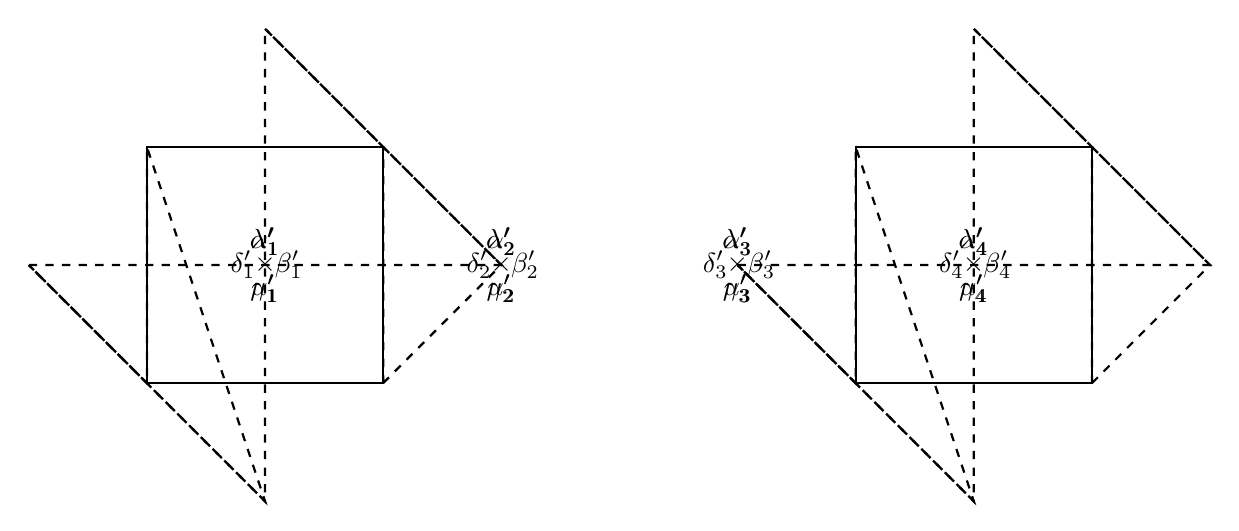
\begin{tikzpicture}[scale=1.5]

        % Define coordinates for the left part of the figure
        \coordinate (A) at (0,0);
        \coordinate (B) at (2,0);
        \coordinate (C) at (2,2);
        \coordinate (D) at (0,2);
        \coordinate (E) at (-1,1);
        \coordinate (F) at (3,1);
        \coordinate (G) at (1,3);
        \coordinate (H) at (1,-1);

        % Draw the left part of the figure
        \draw[thick] (A) -- (B) -- (C) -- (D) -- cycle;
        \draw[thick,dashed] (E) -- (F) -- (G) -- (H) -- cycle;
        \draw[thick,dashed] (A) -- (E) -- (H) -- (D) -- cycle;
        \draw[thick,dashed] (B) -- (F) -- (G) -- (C) -- cycle;

        % Define coordinates for the right part of the figure
        \coordinate (A') at (6,0);
        \coordinate (B') at (8,0);
        \coordinate (C') at (8,2);
        \coordinate (D') at (6,2);
        \coordinate (E') at (5,1);
        \coordinate (F') at (9,1);
        \coordinate (G') at (7,3);
        \coordinate (H') at (7,-1);

        % Draw the right part of the figure
        \draw[thick] (A') -- (B') -- (C') -- (D') -- cycle;
        \draw[thick,dashed] (E') -- (F') -- (G') -- (H') -- cycle;
        \draw[thick,dashed] (A') -- (E') -- (H') -- (D') -- cycle;
        \draw[thick,dashed] (B') -- (F') -- (G') -- (C') -- cycle;

        % Add labels and annotations
        \node at (1,1) {$\times$};
        \node at (3,1) {$\times$};
        \node at (5,1) {$\times$};
        \node at (7,1) {$\times$};

        \node at (1,1) [above] {$\alpha_1'$};
        \node at (3,1) [above] {$\alpha_2'$};
        \node at (5,1) [above] {$\alpha_3'$};
        \node at (7,1) [above] {$\alpha_4'$};

        \node at (1,1) [right] {$\beta_1'$};
        \node at (3,1) [right] {$\beta_2'$};
        \node at (5,1) [right] {$\beta_3'$};
        \node at (7,1) [right] {$\beta_4'$};

        \node at (1,1) [below] {$\gamma_1'$};
        \node at (3,1) [below] {$\gamma_2'$};
        \node at (5,1) [below] {$\gamma_3'$};
        \node at (7,1) [below] {$\gamma_4'$};

        \node at (1,1) [left] {$\delta_1'$};
        \node at (3,1) [left] {$\delta_2'$};
        \node at (5,1) [left] {$\delta_3'$};
        \node at (7,1) [left] {$\delta_4'$};

        \node at (1,1) [above] {$\lambda_1'$};
        \node at (3,1) [above] {$\lambda_2'$};
        \node at (5,1) [above] {$\lambda_3'$};
        \node at (7,1) [above] {$\lambda_4'$};

        \node at (1,1) [below] {$\mu_1'$};
        \node at (3,1) [below] {$\mu_2'$};
        \node at (5,1) [below] {$\mu_3'$};
        \node at (7,1) [below] {$\mu_4'$};

    \end{tikzpicture}
    \caption{Left: Sketch of a $3\times3$ quadrilateral mesh, or equivalently, Kokotsakis polyhedron with a quadrangular base. The flexibility only relies on a smaller area marked in dashed lines; Right: A flexible mesh with fixed angles $\lambda_i', \gamma_i', \mu_i', \delta_i'$, which are well-defined by vector products and $\arccos$ function. The flexible angles $\alpha_i'$ and its complement (not shown) $\alpha_i=\pi-\alpha_i'$ are dihedral angles between the central planar panel and surrounding planar panels, which are rigorously defined in Appendix \ref{dfnang}.}
    \label{fig:flexible_mesh}
\end{figure}

\end{document}